\section{Shortcuts}

\subsection{Beamer box colors}

\setbeamercolor{block title}{use=structure,fg=white,bg=black!75!black}
\setbeamercolor{block title}{use=structure,fg=white,bg=blue!75!black}
\setbeamercolor{block title}{use=structure,fg=white,bg=purple!75!black}
\setbeamercolor{block title}{use=structure,fg=white,bg=cyan!75!black}
\setbeamercolor{block title}{use=structure,fg=white,bg=orange!75!black}

\subsection{Colored line}
{\color{blue} \rule{\linewidth}{1mm}}

\subsection{Line break}
\hfill \break

\subsection{Picture environment}
\begin{figure}[c]
    \centering
    \caption{Tabela verdade para uma proposição composta $H(p,q,r)$.}
    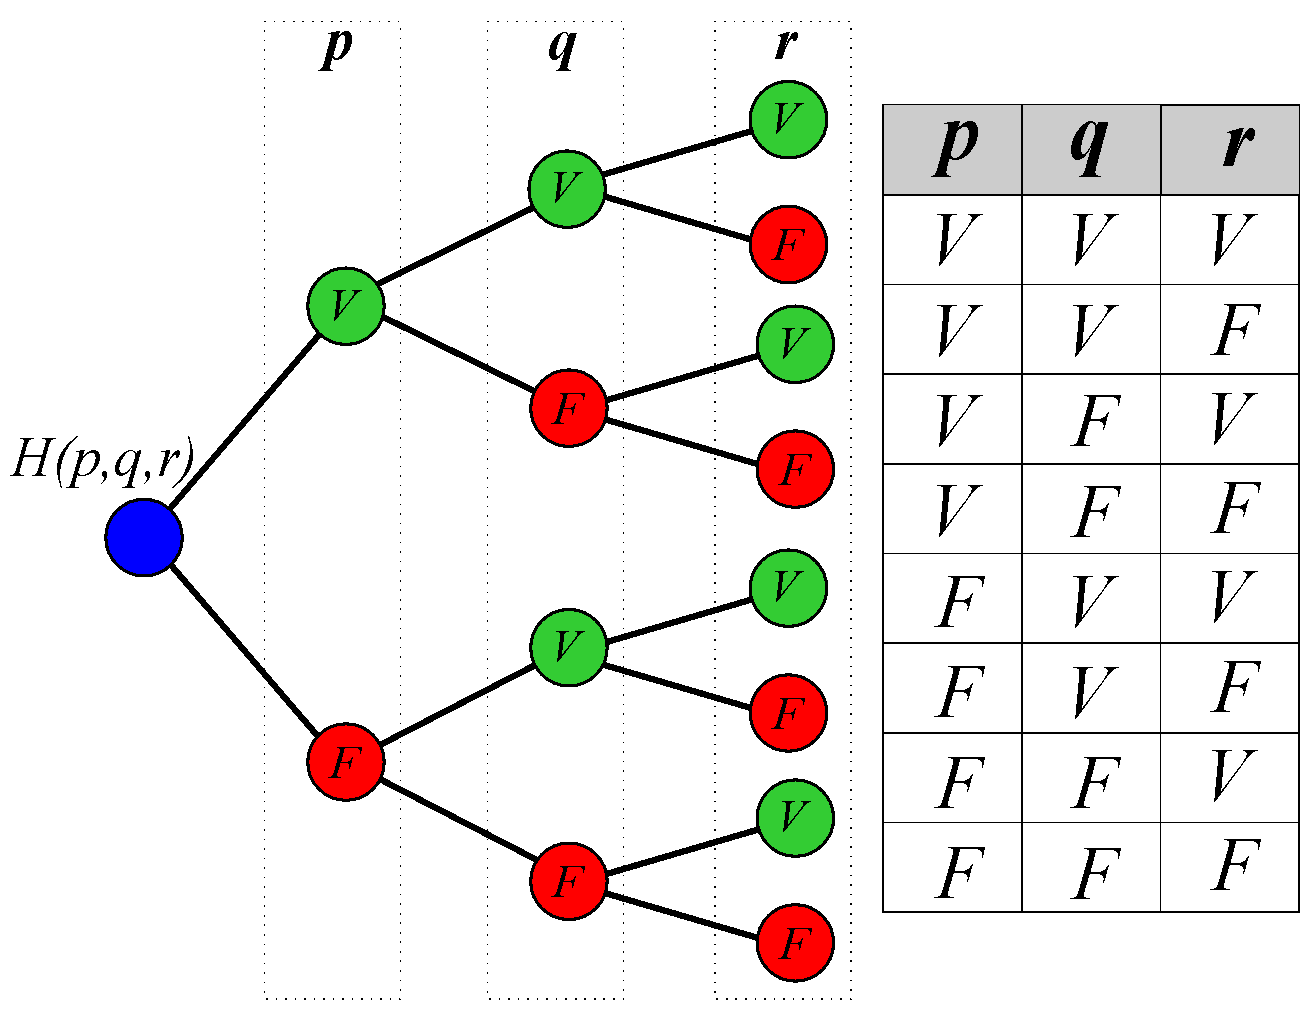
\includegraphics[scale=0.30]{TT4.png}
    \label{fig:tabela-verdade3}
\end{figure}

\subsection{Set background color of the frame - insert immediately outside the frame}
{
    \setbeamercolor{background canvas}{bg=black!15!white}
    \setbeamercolor{background canvas}{bg=yellow!20}
    \begin{frame}
        
    \end{frame}
}

\subsection{Nice box with tcolorbox}
\begin{tcolorbox}[colback=blue!5,colframe=blue!75!black,title=My title]
\begin{tcolorbox}[colback=blue!5,colframe=blue!75!black,title=My title]
    My cool formalization
    \tcblower
    $\displaystyle\sum\limits_{i=1}^n i = \frac{n(n+1)}{2}$ \\
    \textcolor{red}{Text in RED!!}
\end{tcolorbox}

\subsection{Set a background picture - insert inside a block environment}
\usepackage{tikz}
\usetikzlibrary{positioning}

\begin{tikzpicture}[remember picture,overlay]
    \node[above right, inner xsep=0pt, inner ysep=-30pt] at (current page.south west)
    {
        
\includegraphics[width=\paperwidth]{back2.png}
    };
\end{tikzpicture}

\subsection{Several columns with an enumerate environment\setbeamercovered{invisible}}
\setbeamercolor{enumerate item}{fg=red!80!black}
\setbeamertemplate{enumerate items}[default]
\begin{exampleblock}{1. Identifique os itens abaixo que não são fórmulas da lógica proposicional.}
    \begin{columns}[T]
        \begin{column}{0.15\textwidth}
            \begin{enumerate}[\bf a.]
                \item $pq$
                \item $PQ$
                \item $PQ \lnot$
                \item $\lnot PQ$
            \end{enumerate}
        \end{column}
        %
        \hspace*{-5mm}
        %
        \begin{column}{0.15\textwidth}
            \begin{enumerate}[\bf a.]
                \addtocounter{enumi}{4}
                \item $p \land q$
                \item $P \lor Q$
                \item $PQ \land$
                \item $\lor PQ$
            \end{enumerate}
        \end{column}
        %
        \hspace*{-5mm}
        %
        \begin{column}{0.20\textwidth}
            \begin{enumerate}[\bf a.]
                \addtocounter{enumi}{8}
                \item $p \rightarrow q$
                \item $PQ \rightarrow$
                \item $\rightarrow PQ \lnot$
                \item $P \rightarrow Q \rightarrow $
            \end{enumerate}
        \end{column}
        %
    \end{columns}
\end{exampleblock}